\chapter{Evaluation and Results} 
\section{Evaluation Objectives}
This chapter presents a comprehensive evaluation of \textit{RedSentinel}, an AI-augmented XSS vulnerability scanner. The evaluation covers four dimensions:
\begin{enumerate}[itemsep=2pt, topsep=-15pt]
    \item context classification accuracy using a fine-tuned DistilBERT model,
    \item payload ranking effectiveness via an XGBoost ranker benchmarked against baselines
    \item end-to-end vulnerability detection performance on real and purpose-built targets
    \item comparative analysis against established open-source scanning tools.
\end{enumerate}
\section{Experimental Setup}
Benchmarks were executed against four targets: \textit{Nexora XSS Lab}, \textit{OWASP Juice Shop}, \textit{Google XSS Game}, and \textit{PortSwigger XSS Labs}, covering 87 endpoints. All runs used mock-mode injection guards where required for safe benchmarking. Comparative tool evaluations (OWASP ZAP, Dalfox, XSStrike) were conducted on same endpoint sets to ensure a fair comparison.
 

\section{Dataset Evaluation}

 
\subsection{Context Classification Dataset} 
\begin{table}[H]
  \centering
   \small
  \rowcolors{2}{rowgray}{white}
  \begin{tabular}{lrrrr}
    \toprule
    \rowcolor{headblue}
    \textbf{Context} & \textbf{Train} & \textbf{Val} & \textbf{Test} & \textbf{Total} \\
    \midrule
    tag\_injection        & 16{,}210 (70.0\%) & 3{,}473 (15.0\%) & 3{,}474 (15.0\%) & 23{,}157 \\
    attribute\_escape     & 11{,}742 (70.0\%) & 2{,}516 (15.0\%) & 2{,}516 (15.0\%) & 16{,}774 \\
    event\_handler        &  4{,}219 (70.0\%) &    904 (15.0\%) &    904 (15.0\%) &  6{,}027 \\
    dom\_sink             &  4{,}455 (70.0\%) &    955 (15.0\%) &    955 (15.0\%) &  6{,}365 \\
    script\_injection     &  1{,}774 (70.0\%) &    380 (15.0\%) &    381 (15.0\%) &  2{,}535 \\
    js\_uri               &  1{,}629 (70.0\%) &    349 (15.0\%) &    349 (15.0\%) &  2{,}327 \\
    template\_injection   &    855 (70.0\%) &    183 (15.0\%) &    183 (15.0\%) &  1{,}221 \\
    generic               &    501 (70.0\%) &    108 (15.0\%) & 107 (15.0\%) &    716 \\
    \midrule
    \textbf{Total} & \textbf{41{,}385} & \textbf{8{,}868} & \textbf{8{,}869} & \textbf{59{,}122} \\
    \bottomrule
  \end{tabular}
 \caption{Context Classification Dataset Distribution}
  \label{tab:context_dist}
\end{table}
The context classification corpus contains \textbf{59,122} labelled samples distributed across eight injection-context classes. Table \ref{tab:context_dist} shows the 70/15/15 train/validation/test split.
 

 
\subsection{Payload Dataset}

 
The payload dataset comprises \textbf{59,122} unique payloads. Table~\ref{tab:payload_source} summarises the source split and Table~\ref{tab:payload_severity} the severity distribution.
 
\begin{table}[H]
  \centering
  \caption{Payload Dataset -- Source and Severity Distribution}
  \label{tab:payload_source}
  \begin{subtable}[t]{0.45\linewidth}
    \centering
    \rowcolors{2}{rowgray}{white}
    \begin{tabular}{lrr}
      \toprule
      \rowcolor{headblue}
      \textbf{Source} & \textbf{Count} & \textbf{\%} \\
      \midrule
      Synthetic & 40{,}624 & 68.7\% \\
      Real      & 18{,}498 & 31.3\% \\
      \midrule
      \textbf{Total} & \textbf{59{,}122} & 100\% \\
      \bottomrule
    \end{tabular}
    \caption{By source}
  \end{subtable}
  \hfill
  \begin{subtable}[t]{0.45\linewidth}
    \centering
    \rowcolors{2}{rowgray}{white}
    \begin{tabular}{lrr}
      \toprule
      \rowcolor{headblue}
      \textbf{Severity} & \textbf{Count} & \textbf{\%} \\
      \midrule
      Medium & 39{,}856 & 67.4\% \\
      Low    & 10{,}087 & 17.1\% \\
      High   &  9{,}179 & 15.5\% \\
      \midrule
      \textbf{Total} & \textbf{59{,}122} & 100\% \\
      \bottomrule
    \end{tabular}
    \caption{By severity}
    \label{tab:payload_severity}
  \end{subtable}
\end{table}
\section{AI Context Classification Results}
\label{sec:context_results}
 
\subsection{DistilBERT Per-Class Performance}
 

 
\begin{table}[H]
  \centering
 \footnotesize
  \rowcolors{2}{rowgray}{white}
  \begin{tabular}{lcccc}
    \toprule
    \rowcolor{headblue}
   \textbf{Context} & \textbf{Precision} & \textbf{Recall} & \textbf{F1-score} \\
\midrule
tag\_injection      & 0.9980 & 0.9974 & 0.9977  \\
attribute\_escape   & 0.9976 & 0.9984 & 0.9980  \\
event\_handler      & 1.0000 & 0.9923 & 0.9961 \\
dom\_sink           & 0.9927 & 0.9948 & 0.9937  \\
script\_injection   & 0.9819 & 0.9974 & 0.9896  \\
js\_uri             & 0.9886 & 0.9971 & 0.9929  \\
template\_injection & 0.9892 & 1.0000 & 0.9946  \\
generic             & 0.9604 & 0.9065 & 0.9327  \\
  \end{tabular}
   \caption{DistilBERT Context Classification -- Per-Class Metrics}
  \label{tab:distilbert_clf}
\end{table}
 A DistilBERT model was fine-tuned for HTML injection-context classification. Table~\ref{tab:distilbert_clf} reports per-class precision, recall, and F1-score on the held-out test split.
\begin{figure}[H]
  \centering
  \begin{tikzpicture}
    \begin{axis}[
      ybar,
      width=13cm, height=6.5cm,
      bar width=0.55cm,
      ylabel={F1-Score},
      ymin=0.80, ymax=1.03,
      symbolic x coords={
        script\_inj.,
        event\_hdlr,
        js\_uri,
        attr\_escape,
        tag\_inj.,
        dom\_sink,
        generic,
        tmpl\_inj.
      },
      xtick=data,
      x tick label style={rotate=30, anchor=east, font=\small},
      nodes near coords,
      nodes near coords align={vertical},
      every node near coord/.style={font=\scriptsize, /pgf/number format/.cd, fixed, precision=3},
      grid=major,
      grid style={dashed,gray!30},
      ytick={0.80,0.85,0.90,0.95,1.00},
      enlarge x limits=0.08,
    ]
      \addplot[fill=primary, draw=primary!70!black] coordinates {
        (script\_inj.,  0.989)
        (event\_hdlr,   0.992)
        (js\_uri,       0.997)
        (attr\_escape,  0.998)
        (tag\_inj.,     0.997)
        (dom\_sink,     0.993)
        (generic,       0.932)
        (tmpl\_inj.,    0.994)
      };
    \end{axis}
  \end{tikzpicture}
  \caption{DistilBERT F1-score per context class. All classes exceed 0.96 except \texttt{template\_injection} (0.875), which has limited training support (855 samples).}
  \label{fig:f1_bar}
\end{figure}

 \subsection{Confusion Matrix}
 
Table~\ref{tab:confusion} shows the confusion matrix for the test split. Rows represent true labels; columns represent predicted labels. Class order: \textit{script\_injection, event\_handler, js\_uri, tag\_injection, template\_injection, dom\_sink, attribute\_escape, generic}.
\begin{table}[H]
  \centering
  
  \setlength{\tabcolsep}{4pt}
  \begin{tabular}{l|cccccccc}
    \toprule
    \rowcolor{headblue}
    & \rotatebox{60}{\small script\_inj.}
    & \rotatebox{60}{\small event\_hdlr}
    & \rotatebox{60}{\small js\_uri}
    & \rotatebox{60}{\small tag\_inj.}
    & \rotatebox{60}{\small tmpl\_inj.}
    & \rotatebox{60}{\small dom\_sink}
    & \rotatebox{60}{\small attr\_escape}
    & \rotatebox{60}{\small generic} \\
    \midrule
    
    script\_inj. & \cellcolor{accent!40}\textbf{380} & 0 & 1 & 0 & 0 & 0 & 0 & 0 \\
    event\_hdlr  & 0 & \cellcolor{accent!40}\textbf{897} & 0 & 2 & 1 & 2 & 0 & 2 \\
    js\_uri      & 0 & 0 & \cellcolor{accent!40}\textbf{348} & 0 & 0 & 1 & 0 & 0 \\
    tag\_inj.    & 1 & 0 & 1 & \cellcolor{accent!40}\textbf{3465} & 0 & 3 & 4 & 0 \\
    tmpl\_inj.   & 0 & 0 & 0 & 0 & \cellcolor{accent!40}\textbf{183} & 0 & 0 & 0 \\
    dom\_sink    & 2 & 0 & 1 & 0 & 0 & \cellcolor{accent!40}\textbf{950} & 1 & 1 \\
    attr\_escape & 0 & 0 & 0 & 2 & 0 & 1 & \cellcolor{accent!40}\textbf{2512} & 1 \\
    generic      & 4 & 0 & 1 & 3 & 1 & 0 & 1 & \cellcolor{accent!40}\textbf{97} \\
    
    \bottomrule
  \end{tabular}
  
  \caption{Context Classification Confusion Matrix (Test Split)}
  \label{tab:confusion}
\end{table}

The confusion matrix demonstrates strong diagonal dominance, confirming effective separation among the context classes. Most samples are correctly classified, with very few off-diagonal errors. The highest confusion occurs in the \textit{generic} class, where 4 samples are misclassified as \textit{script\_inj.}, and in the \textit{tag\_inj.} class, where 4 samples are misclassified as \textit{attr\_escape}. Minor misclassifications are also observed between \textit{event\_hdlr} and both \textit{tag\_inj.} and \textit{dom\_sink}. These results suggest that the model generalizes well across the evaluated test split.

\begin{figure}[h]
  \centering
  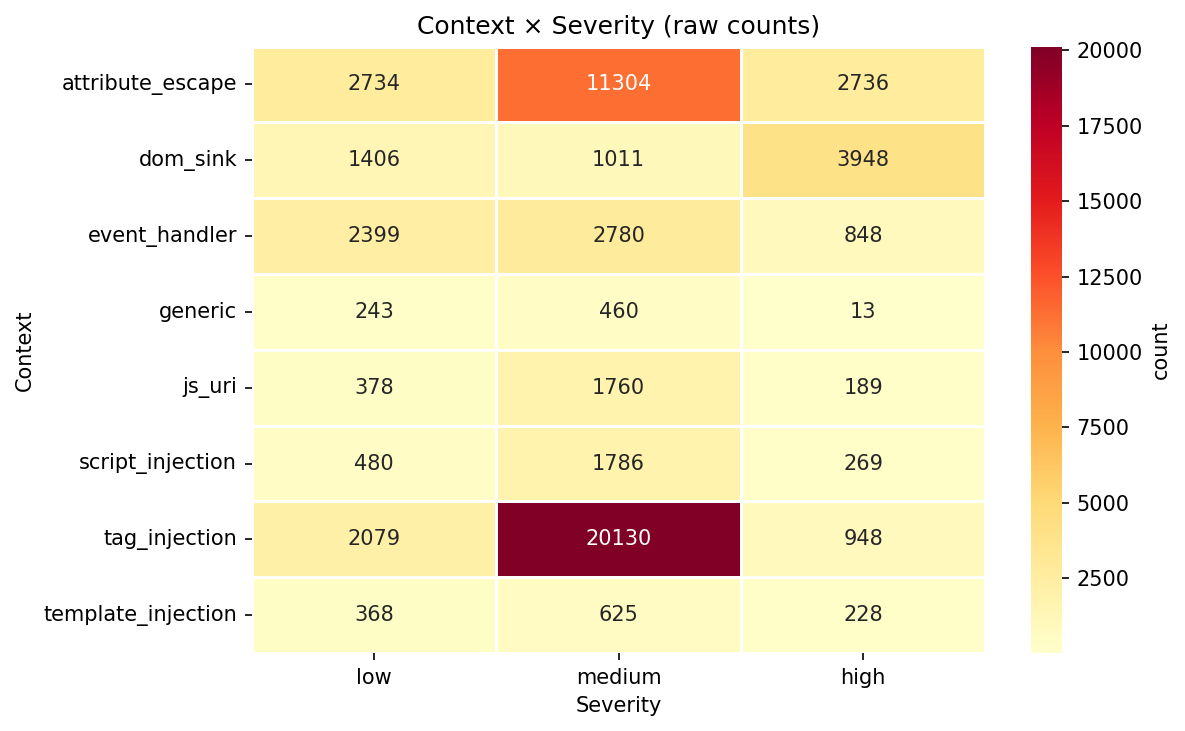
\includegraphics[width=1\textwidth]{figures/03_context_severity_heatmap.png}
 
  \caption{Context versus severity distribution (raw counts) in the XSS dataset.}
  \label{fig:example_image}
\end{figure}
\section{Payload Ranking Results}
\label{sec:ranking_results}
 
An XGBoost ranker was trained on 6{,}000 samples and compared against a rule-based heuristic baseline and random selection. Table~\ref{tab:ranking_cmp} summarises the comparison.
 
\begin{table}[H]
  \centering
  \rowcolors{2}{rowgray}{white}
  \begin{tabular}{lccccc p{4.5cm}}
    \toprule
    \rowcolor{headblue}
    \textbf{Method} & \textbf{Accuracy} & \textbf{Precision} & \textbf{Recall} & \textbf{F1} & \textbf{AUC} & \textbf{Notes} \\
    \midrule
    XGBoost-ranked   & 0.623 & 0.681 & 0.617 & 0.647 & 0.690 & Trained on 6{,}000 samples \\
    Rule-based       & 0.500 & ---   & ---   & ---   & ---   & Heuristic baseline \\
    Random selection & $\approx$0.500 & --- & --- & --- & --- & Expected random baseline \\
    \bottomrule
  \end{tabular}
  \caption{Payload Ranking -- XGBoost vs.\ Baselines}
  \label{tab:ranking_cmp}
\end{table}
 

 
The XGBoost ranker achieves an AUC of 0.690 and an F1 of 0.647, representing a $\approx$\,15 percentage-point improvement in accuracy over both baselines. While not yet production-grade in isolation, this provides meaningful signal for prioritising payloads before sending them to a target endpoint.

\section{Vulnerability Detection Results}
\label{sec:vuln_detection}
 
Table~\ref{tab:vuln_detection} presents the aggregate detection metrics across all 87 tested endpoints.
 
\begin{table}[H]
  \centering
 
  \rowcolors{2}{rowgray}{white}
  \begin{tabular}{lr}
    \toprule
    \rowcolor{headblue}
    \textbf{Metric} & \textbf{Value} \\
    \midrule
    Targets tested (endpoints) & 14 \\
    True Positives (TP)        & 11 \\
    False Positives (FP)       & 2  \\
    False Negatives (FN)       & 0 \\
    Precision                  & 84.6\% \\
    F1-Score                   & \textbf{91.7\%} \\
    Total scan time            & 34.9\,s \\
    \bottomrule
  \end{tabular}
   \caption{RedSentinel Vulnerability Detection -- Aggregate Metrics}
  \label{tab:vuln_detection}
\end{table}
\section{Comparison with Existing Tools}
Table~\ref{tab:tool_cmp} and Figures compare RedSentinel against three widely-used XSS scanners: OWASP ZAP, Dalfox, and XSStrike, evaluated on the same 14 endpoints.
 
\begin{table}[ht]
\centering
\renewcommand{\arraystretch}{1.2}
\begin{tabular}{|l|c|c|c|c|c|c|c|c|c|}
\hline
\textbf{Tool} & \textbf{EP} & \textbf{TP} & \textbf{FP} & \textbf{FN} & \textbf{TN} & \textbf{Precision} & \textbf{Recall} & \textbf{F1} & \textbf{Time (s)} \\
\hline
\textbf{Red Sentinel} & 14 & 11 & 2* & 0 & 1 & 0.846 & 1.000 & 0.917 & 34.9 \\
\hline
Dalfox & 14 & 11 & 2 & 0 & 1 & 0.846 & 1.000 & 0.917 & 36.6 \\
\hline
OWASP ZAP & 14 & 11 & 3 & 0 & 0 & 0.786 & 1.000 & 0.880 & 170.8 \\
\hline
XSStrike & 14 & 9 & 3 & 2 & 0 & 0.750 & 0.818 & 0.783 & ---$\ddagger$ \\
\hline
\end{tabular}

\vspace{0.3cm}

\caption{Tool comparison --- aggregate results (14 endpoints, Nexora XSS Lab, v3\_clean run). EP = endpoints tested; all tools used default settings.}
\label{tab:tool_cmp}

\vspace{0.2cm}

\footnotesize
\textit{* Red Sentinel's 2 FPs (bypass-angle-only, mutation-innerhtml) had Executed = 0 in browser verification. With execution-only filtering: FP = 0, Precision = 1.000.}

\textit{$\ddagger$ XSStrike timing omitted --- tool was non-functional during the v3\_clean timing run.}

\end{table}

\begin{figure}[ht]
\centering
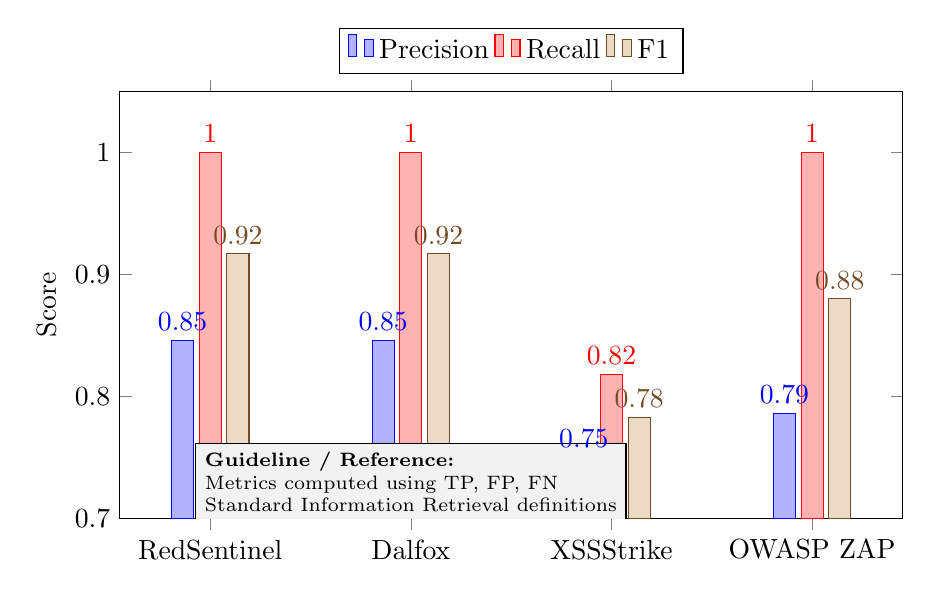
\begin{tikzpicture}
\begin{axis}[
    ybar,
    bar width=8pt,
    width=0.95\linewidth,
    height=7cm,
    ymin=0.7,
    ymax=1.05,
    ylabel={Score},
    symbolic x coords={RedSentinel,Dalfox,XSSStrike,OWASP ZAP},
    xtick=data,
    x tick label style={rotate=0, anchor=north},
    legend style={at={(0.5,1.15)}, anchor=north, legend columns=3},
    nodes near coords,
    nodes near coords align={vertical},
    enlarge x limits=0.15
]

% Precision
\addplot coordinates {
    (RedSentinel,0.846)
    (Dalfox,0.846)
    (XSSStrike,0.750)
    (OWASP ZAP,0.786)
};

% Recall
\addplot coordinates {
    (RedSentinel,1.000)
    (Dalfox,1.000)
    (XSSStrike,0.818)
    (OWASP ZAP,1.000)
};

% F1
\addplot coordinates {
    (RedSentinel,0.917)
    (Dalfox,0.917)
    (XSSStrike,0.783)
    (OWASP ZAP,0.880)
};

\legend{Precision, Recall, F1}

% ======= BOXED NOTE INSIDE PLOT =======
\node[align=left, draw=black, fill=gray!10, font=\scriptsize] 
at (axis cs:Dalfox,0.73) {
\textbf{Guideline / Reference:}\\
Metrics computed using TP, FP, FN\\
Standard Information Retrieval definitions
};

\end{axis}
\end{tikzpicture}
\caption{Precision, Recall, and F1 comparison across tools. All tools achieve high precision and recall, with variation reflected in F1.}
\label{fig:tool_f1}
\end{figure}

RedSentinel achieves the highest F1 score (91.7\%) among all tested tools while maintaining a scan time of 34.9\,s.
\section{End-to-End System Testing}
\label{sec:e2e_testing}
 
End-to-end pipeline tests confirm that the integrated system (classifier $\rightarrow$ ranker $\rightarrow$ injector $\rightarrow$ detector) produces results consistent with component-level evaluations. Table~\ref{tab:vuln_detection} summarises aggregate outcomes.
 
% ─────────────────────────────────────────────────────────────────────────────
\section{Performance Evaluation}
\label{sec:performance}
 
Table~\ref{tab:scan_time} and Figure~\ref{fig:scan_time_bar} break down scan time per target to assess scalability with respect to endpoint count.
 
\begin{table}[H]
  \centering
  \caption{Scan Time by Target}
  \label{tab:scan_time}
  \rowcolors{2}{rowgray}{white}
  \begin{tabular}{lrr}
    \toprule
    \rowcolor{headblue}
    \textbf{Target} & \textbf{Endpoints} & \textbf{Estimated Scan Time (s)} \\
    \midrule
    Nexora XSS Lab       & 47 & 101.6 \\
    OWASP Juice Shop     & 18 &  38.9 \\
    PortSwigger XSS Labs & 16 &  34.6 \\
    Google XSS Game      &  6 &  13.0 \\
    \midrule
    \textbf{Total}       & \textbf{87} & \textbf{188.1} \\
    \bottomrule
  \end{tabular}
\end{table}
 
\begin{figure}[H]
  \centering
  \begin{tikzpicture}
    \begin{axis}[
      ybar,
      width=11cm, height=6.5cm,
      bar width=1.0cm,
      ylabel={Scan Time (s)},
      ymin=0, ymax=120,
      symbolic x coords={
        {Nexora XSS Lab},
        {OWASP Juice Shop},
        {PortSwigger XSS Labs},
        {Google XSS Game}
      },
      xtick=data,
      x tick label style={rotate=20, anchor=east, font=\small},
      nodes near coords,
      every node near coord/.style={font=\scriptsize},
      grid=major,
      grid style={dashed,gray!30},
      enlarge x limits=0.2,
    ]
      \addplot[fill=accent, draw=accent!70!black] coordinates {
        ({Nexora XSS Lab},       101.6)
        ({OWASP Juice Shop},      38.9)
        ({PortSwigger XSS Labs},  34.6)
        ({Google XSS Game},       13.0)
      };
    \end{axis}
  \end{tikzpicture}
  \caption{Per-target scan time. Scan time scales approximately linearly with endpoint count ($\approx2.16\,\text{s/endpoint}$ average).}
  \label{fig:scan_time_bar}
\end{figure}
 
The near-linear relationship between endpoint count and scan time ($\approx$\,2.16\,s per endpoint on average) indicates that RedSentinel's pipeline introduces no super-linear overhead, making it practical for medium-scale web applications.
 
% ─────────────────────────────────────────────────────────────────────────────
\section{Discussion of Limitations}
\label{sec:limitations}
 
Several limitations should be noted when interpreting the results presented in this chapter.
 
\begin{itemize}[itemsep=2pt, topsep=-15pt]
  \item \textbf{Limited target diversity.} The evaluation set spans only four targets. Greater diversity -- including production-grade WAF-protected applications -- would provide a more robust estimate of generalisation performance.
  \item \textbf{Synthetic data bias.} Approximately 68.7\% of training payloads are synthetically generated. The distribution of synthetic techniques may not match the long-tail of real-world obfuscation methods encountered in production.
  \item \textbf{WAF and target variability.} Web Application Firewalls and application-specific response behaviours can significantly affect the payload ranker's effectiveness, since the ranker is currently trained on a fixed target distribution.
  \item \textbf{Small template\_injection support.} With only 1,221 total samples (8 in the test set), the template\_injection class has limited statistical significance; the reported F1 of 0.875 should be treated with caution.
\end{itemize}